\subsection{Erzeugung}

\begin{iframe}
	\begin{columns}
		\begin{column}{0.48\textwidth}
			\begin{figure}
				\feynmandiagram[large,horizontal=a to b] {
					i1 -- [fermion,edge label=\(e^-\)] a -- [fermion,edge label=\(e^+\)] i2,
					a -- [boson,edge label=\(\gamma\)] b,
					f1 -- [fermion,edge label'=\(\overline f\)] b -- [fermion,edge label'=\(f\)] f2,
				};
				\caption*{$e^+e^$-Vernichtung über $\gamma$ \cite{perkins}}
			\end{figure}
		\end{column}
		\begin{column}{0.48\textwidth}
			\begin{figure}
				\feynmandiagram[large,horizontal=a to b] {
					i1 -- [fermion,edge label=\(e^-\)] a -- [fermion,edge label=\(e^+\)] i2,
					a -- [boson,edge label=\(Z^0\)] b,
					f1 -- [fermion,edge label'=\(\overline f\)] b -- [fermion,edge label'=\(f\)] f2,
				};
				\caption*{$e^+e^$-Vernichtung über $Z^0$ \cite{perkins}}
			\end{figure}
		\end{column}
	\end{columns}
\end{iframe}

\note[itemize] {
	\item W/Z-Boson durch Antilepton+Lepton/AntiQuark+Quark Reaktion
	\item kollidierende Teilchenstrahlen
	\item feynman diagram
	\item Zeit nach rechts
	\item Antiteilchen Zeitlich invers (Aus Dirac-Gleichung (Schrödinger gleichung mit eingesetzter Impuls/Energie Relation wirkt auf vier komponentigen Dirac Spinor) ergeben sich positive und negative Lösungen für die Energie) (bzw. Klein Gordon Gleichung (entkoppelt)) nach Stückelberg-Feynman-Interpretation, bsplw. E-Feld $e^-$ vs $e^+$ mit anderer Richtung ist gleich. (Dirac sagte Antiteilchen vorher/definierte, wobei negative Energien besetzt sind und Löcher sich ausbreiten basierend auf Pauli-Ausschlussprinzip, da Bosonen nicht gehorchen => reverse Zeit Interpretation)
	\item über $\gamma $oder $Z$ zu Fermion und Antifermion paar.
	\item bei passender Energie\ approx $M_Z$  dominiert $Z^0$, aus QFT+Feynmanregeln
}

\begin{iframe}
	\begin{itemize}
		\item Schwerpunktsenergie $\sqrt{s} = 2E_e \geq M_\text{Z}c^2 \approx \SI{91.6}{GeV}$
		\pause
		\item $pp$-Kollision: $u + \overline{u} \rightarrow Z^0 $ benötigt $\sqrt{s} \gtrapprox \SI{600}{GeV}$ pro Proton
		\pause
		\item $e^+ + e^- \rightarrow W^+ + W^-$ benötigt $\sqrt{s} \geq 2M_\text{W}c^2 \approx \SI{160.8}{GeV}$
	\end{itemize}
	\note[item]{ 1989 am Stanford Linear Collider und LEP}
	\note[item]{Energie muss in Quarks enthalten sein $\rightarrow$ sehr viel mehr Energie auf Protonen (analog mit d) => e-e+ Kollision einfacher}
	\note[item]{ 1996 am LEP, 50 $\rightarrow$ 86 $\rightarrow$  \SI{104.6}{GeV}}
\end{iframe}

\subsection{Nachweis}
\begin{iframe}
	\framesubtitle{1983 am CERN}
	\begin{figure}
		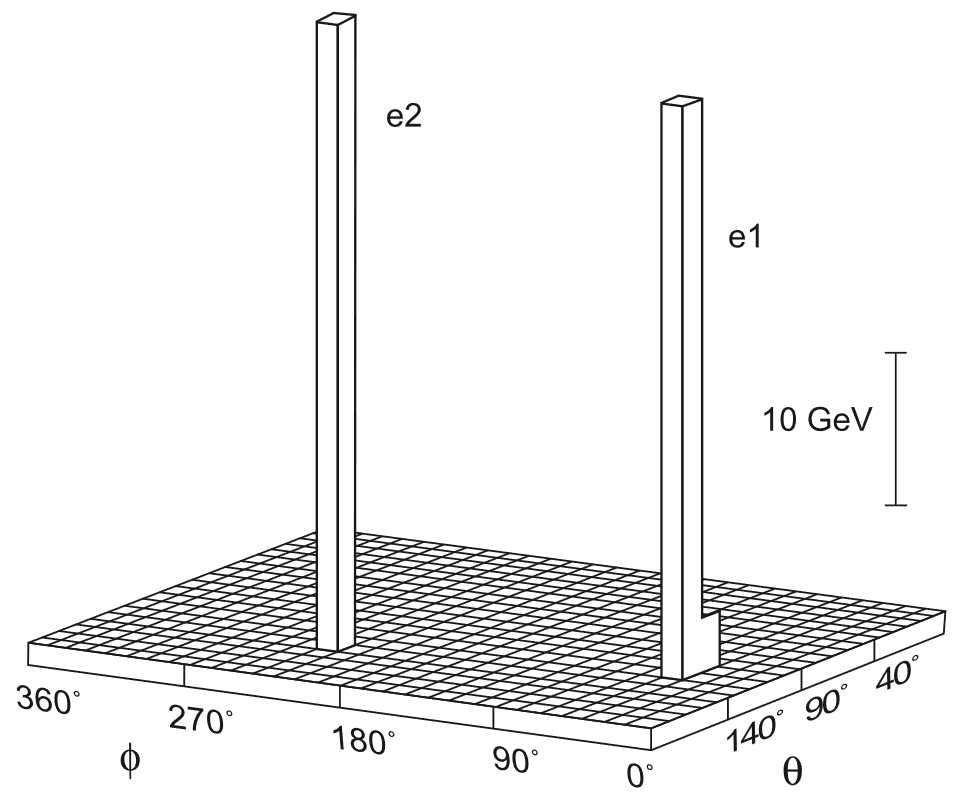
\includegraphics[width=6cm]{img/lego}
		\caption*{$q+\overline{q} \rightarrow Z^0 \rightarrow e^+ + e^-$ \cite{povh}}
	\end{figure}
\end{iframe}

\note[itemize] {
	\item Plane unten sind Kaloriemeterzellen
	\item Energie Summe $=$ Masse $Z^0$
	\item Beispiel Event einer Messung
	\item Winkel 180° => entgegen gesetzte Richtungen

	\item ?Woher sicher, dass $Z^0$ Zerfall?
}

\begin{iframe}
	\framesubtitle{1993 am LEP/CERN}
	\begin{figure}
		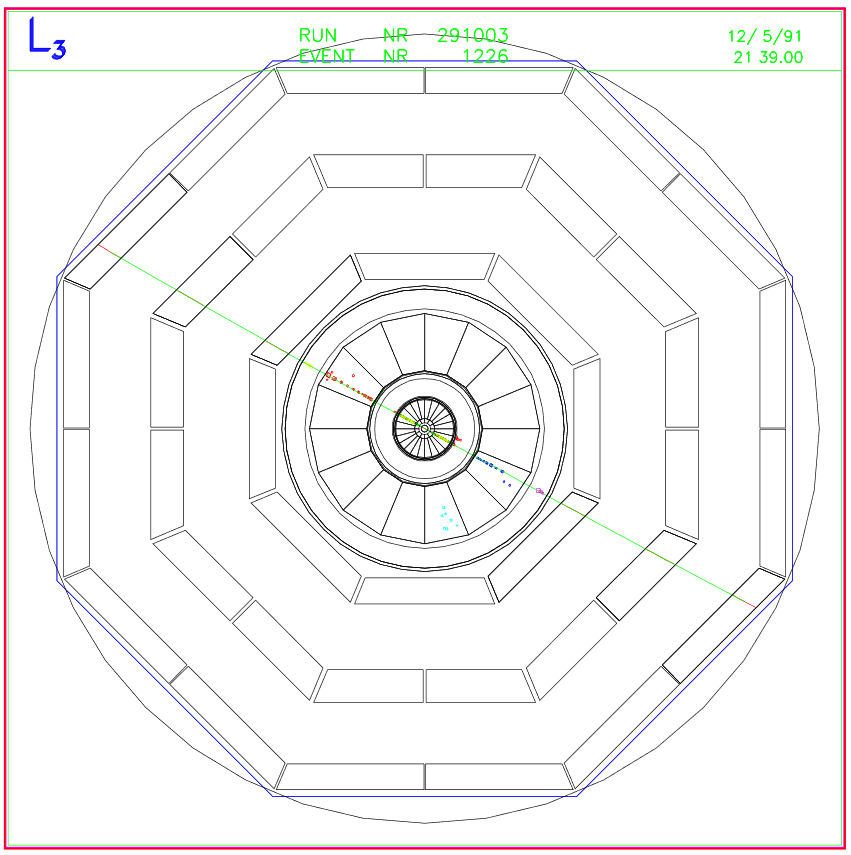
\includegraphics[height=5cm]{img/muon}
		\caption*{$e^- +e^- \rightarrow Z^0 \rightarrow \mu^+ + \mu^-$ \cite{huz0}}
	\end{figure}
\end{iframe}

\note[itemize] {
	\item Beispiel Muon
	\item Winkel 180° => entgegen gesetzte Richtungen
	\item ?Woher sicher, dass $Z^0$ Zerfall?
}

\subsection{Eigenschaften}
\begin{iframe}
	\framesubtitle{Experimentelle Bestimmung}
	\begin{itemize}
		\item Messung: %TODO Graphik!!
		\begin{itemize}
			\item $M_Z = \SI{91.188+-0.002}{GeV/c^2}$
			\item $\Gamma_Z = \SI{2.495+-0.002}{GeV}$
		\end{itemize}
		\pause
		\item Zerfall:
		\begin{align*}
			Z^0 \rightarrow & e^+ + e^- & \SI{3.363+-0.004}{\%} \\
			& \mu^+ + \mu^- & \SI{3.366+-0.007}{\%} \\
			& \tau^+ + \tau^- & \SI{3.370+-0.008}{\%} \\
			& \nu_{e,\mu,\tau}^+ + \overline{\nu}_{e,\mu,\tau} & \SI{20+-0.06}{\%} \\
			& \text{Hadronen} & \SI{69.91+-0.06}{\%} \\
		\end{align*}
	\end{itemize}
\note[item]{Über Wirkungsquerschnitt? src [PD12]}
\note[item]{}
\note[item]{Hadronen (idR. Anti+Quark) nicht unterscheidbar}
\note[item]{Anti+Neutrino schwer detektierbar => \% über $\Gamma_\text{tot}$}
\note[item]{totale Breite = alle Zerfälle Anti+Fermion???}
%\note[item]{$Z^0$ nicht nur ungeladenes $W$-Boson, da }
\end{iframe}

\subsection{Neutrinogenerationen}

\begin{iframe}
	\framesubtitle{Wirkungsquerschnitt}
	\begin{columns}
		\begin{column}{0.48\textwidth}
			\begin{equation*}
				\sigma_f = \sigma_0 \cdot \frac{s\Gamma_Z^2}{(s-M_Z^2)^2 + M_Z^2\Gamma_Z^2}
			\end{equation*}
			mit
			\begin{equation*}
				\sigma_0 = \frac{12\pi}{M_Z^2}\cdot\frac{\Gamma_{i=e}\Gamma_f}{\Gamma_Z^2}
			\end{equation*}
		\end{column}
		\begin{column}{0.48\textwidth}
		\end{column}
	\end {columns}
	\begin{textblock*}{5cm}(7cm,3cm) % {block width} (coords)
				\begin{figure}
				\feynmandiagram[large,horizontal=a to b] {
					i1 -- [fermion,edge label=\(e^-\)] a -- [fermion,edge label=\(e^+\)] i2,
					a -- [boson,edge label=\(Z^0\)] b,
					f1 -- [fermion,edge label'=\(\overline f\)] b -- [fermion,edge label'=\(f\)] f2,
				};
			\end{figure}
		\end{textblock*}
\note[item]{Formel für $\sigma$ Breit-Wigner}
\note[item]{Abhängig von ...}
\note[item]{$\gamma$ unterdrückt}
\end{iframe}

\begin{iframe}
	\framesubtitle{Zerfallsbreite}
	\begin{align*}
		\action<+->{\Gamma_Z&=\sum_f \Gamma_{Z \rightarrow f\bar{f}}\\}
		\action<+->{&= \Gamma_\text{Had}  + \Gamma_\text{Lep}+ \Gamma_\nu\\}
		\action<+->{&= N_C \cdot2\cdot\Gamma_u + N_C\cdot 3\cdot \Gamma_d + 3\cdot\Gamma_e + 3\cdot\Gamma_\nu\\}
		\action<+->{&= 3 \cdot 2\cdot\SI{94.9}{MeV} + 3\cdot3\cdot \SI{122.4}{MeV}+ 3\cdot \SI{83.3}{MeV} + 3\cdot \SI{165.8}{MeV} \\} %TODO fix SI font
		\action<+->{&=\SI{2.42}{GeV}\\}
		\action<+->{&\xrightarrow[\text{korrektur}]{\text{Strahlungs-}}\SI{2.497}{GeV}\\}
	\end{align*}
\note[item]{$\Gamma_f=\frac{G_F M_Z^3}{24\sqrt{2}\pi}\cdot (1+(1-e|Q_f|\sin^2{\theta_W})^2)$}
\note[item]{$G_F$ Fermikonstante}
\note[item]{$Q_f$ Ladung des Fermions}
\note[item]{ Lep: $e^\pm$, $\mu^\pm$, $\tau^\pm$}
\note[item]{ Had: u,c= 2/3; d,s,b=-1/3}
\note[item]{ Neutrinos}
\note[item]{kein top-Quark weil nicht genug Energie aus $Z^0$ ($\approx \SI{175}{ GeV}$)}
\note[item]{Korrekturen aus QFT, höherer Ordungen, Strahlungskorrektur}
\note[item]{Passt mit Unsicherheiten zu Exp. (nicht auf Folie)}
\note[item]{$\Gamma_e/\Gamma_{tot}=3,37\%$ passt auch zu Exp.}
\end{iframe}

\begin{iframe}
	\begin{figure}
		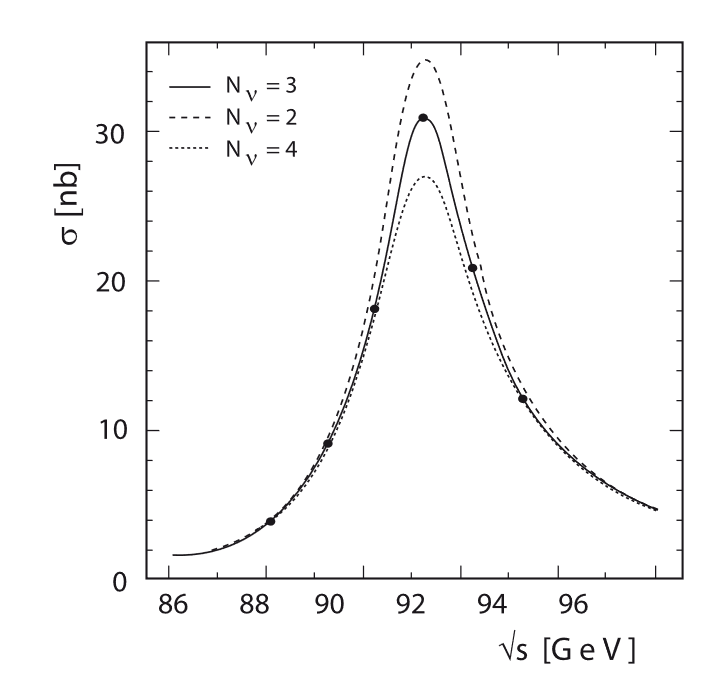
\includegraphics[width=5.5cm]{img/neutrinogen}
		\caption*{Wirkungsquerschnitt $e^+e^-\rightarrow $Hadronen \cite{povh}}
	\end{figure}
	\note[item]{Cern Experiment}
	\note[item]{Schwerpunkt energie gegen Wirkungsquerschnitt}
	\note[item]{Ähnlich der Breit Wigner Funktion aber nicht passend symmetrisch durch Korrekturen höherer Ordnung udn Bremstrahlung durch $e^-$}
	\note[item]{Verschiedene Anzahl-Neutrinogenerationen-Kurven}
	\note[item]{3 Neutrinogenerationen $\rightarrow$ 3 Leptonen 3 Quarks Generationen}
\end{iframe}
%TODO Neutrino generationen
